%!TEX root = ../thesis.tex

\chapter{Results}

This section presents the results obtained by this evaluative study. Performance results for the various frameworks is presented, obtained by measuring the execution time of the implementations. Features of the different frameworks and the portability of the frameworks are presented. Finally, a simple full vector addition implementation in the various frameworks, including both the host and the device code, are presented and evaluated in terms of cyclomatic code complexity for the various frameworks.


\section{Performance}

To measure the performance of all frameworks when performing the N-Body simulation, the execution time was measured when simulating a fixed amount of timesteps for a dynamic range of bodies. The \lstinline{std::chrono} library was used the measure the execution time in milliseconds. To minimize the performance degradation generated by the visualization, the visualization was disabled when the tests were run. The tests were performed in Microsoft Visual Studio 2012 by running the various implementations without the debugger since the debugger drastically degrades the performance.
The code was compiled by Microsoft's Visual C++ 11.0. The specifications for the system that the tests were performed on are listed in table \ref{tab:SystemSpecs}.

\begin{table}[H]

    % General
    \begin{tabularx}{\textwidth}{ |X|X| }
      \hline
      \rowcolor{gray}
      \multicolumn{2}{|c|}{\textbf{General}}\\ \hline
      
      \textbf{Operating system}         & Windows 7 Professional x64 \\ \hline
      \textbf{CPU}                      & Intel Core i7-3770 @ 3.40GHz (8 CPUs) \\ \hline
      \textbf{GPU}                      & NVIDIA GeForce GTX 1050 \\ \hline
      \textbf{RAM}                      & 16 GB\\ \hline
    \end{tabularx}
    
    % GPU Specs
    \begin{tabularx}{\textwidth}{ |X|X| }
      \hline
      \rowcolor{gray}
      \multicolumn{2}{|c|}{\textbf{GPU}}\\ \hline
      
      \textbf{Manufacturer}             & NVIDIA \\ \hline
      \textbf{Model}                    & GeForce GTX 1050 \\ \hline
      \textbf{GPU Architecture}         & Pascal \\ \hline
      \textbf{Compute Capability}       & 6.1 \\ \hline
      \textbf{Global Memory}            & 2048mb \\ \hline
      \textbf{Memory Speed}             & 7 Gbps \\ \hline
      \textbf{Memory Bandwidth}         & 12 GB/sec \\ \hline
      \textbf{No. Multorprocessors}     & 5 \\ \hline
      \textbf{CUDA Cores}               & 640 \\ \hline
      \textbf{Warp size}                & 32 \\ \hline
        
    \end{tabularx}
    
    % Framework specs
    \begin{tabularx}{\textwidth}{ |X|X| }
      \hline
      \rowcolor{gray}
      \multicolumn{2}{|c|}{\textbf{Frameworks}}\\ \hline
      
      \textbf{CUDA}                 & v9.1 \\ \hline
      \textbf{OpenCL}               & v1.2 (NVidia) \\ \hline
      \textbf{DirectX 11}           & 11 \\ \hline
      \textbf{CS Shader Profile}    & CS 5.0 \\ \hline
        
    \end{tabularx}
    
    
\caption{\label{tab:SystemSpecs} System specifications on which the tests were performed.}
\end{table}


%% ===================================== %%
%% Performance tests results tables HERE %%
%% ===================================== %%
% SEQUENTIAL DOES NOT NEED TO FLATTEN THE TREE -> Performance boost
% VAD MÄTA???
%
% * Total exekveringstid                                                              DONE
% * Bar chart med tid per operation (bygga träd, platta ut träd, calc. force osv)     DONE
% * Endast GPU exekveringstid                                                         DONE
% * Sepererade steg (dvs kopiera tbx data mellan kraft/pos beräkning)
%% ===================================== %%

The total execution time of the frameworks are presented in figure \ref{fig:GraphTotExecTime}. The total execution time includes both the part of the algorithm that is executed on the host and the device when simulating N-Body systems in the range $N \in [1024, 20480]$ and was measured by simulating $100$ timesteps for each $N$ without using any visualization. 

\begin{figure}[H]
    \centering
    \includegraphics[width=0.8\textwidth]{Results/Figs/TotalExecutionTime.png}
    \caption{Total execution time}
    \label{fig:GraphTotExecTime}
\end{figure}

The part of the algorithm that is executed on the device, i.e. the force calculation and position update was measured and is presented in figure \ref{fig:GPUStepExecTime}.

\begin{figure}[H]
    \centering
    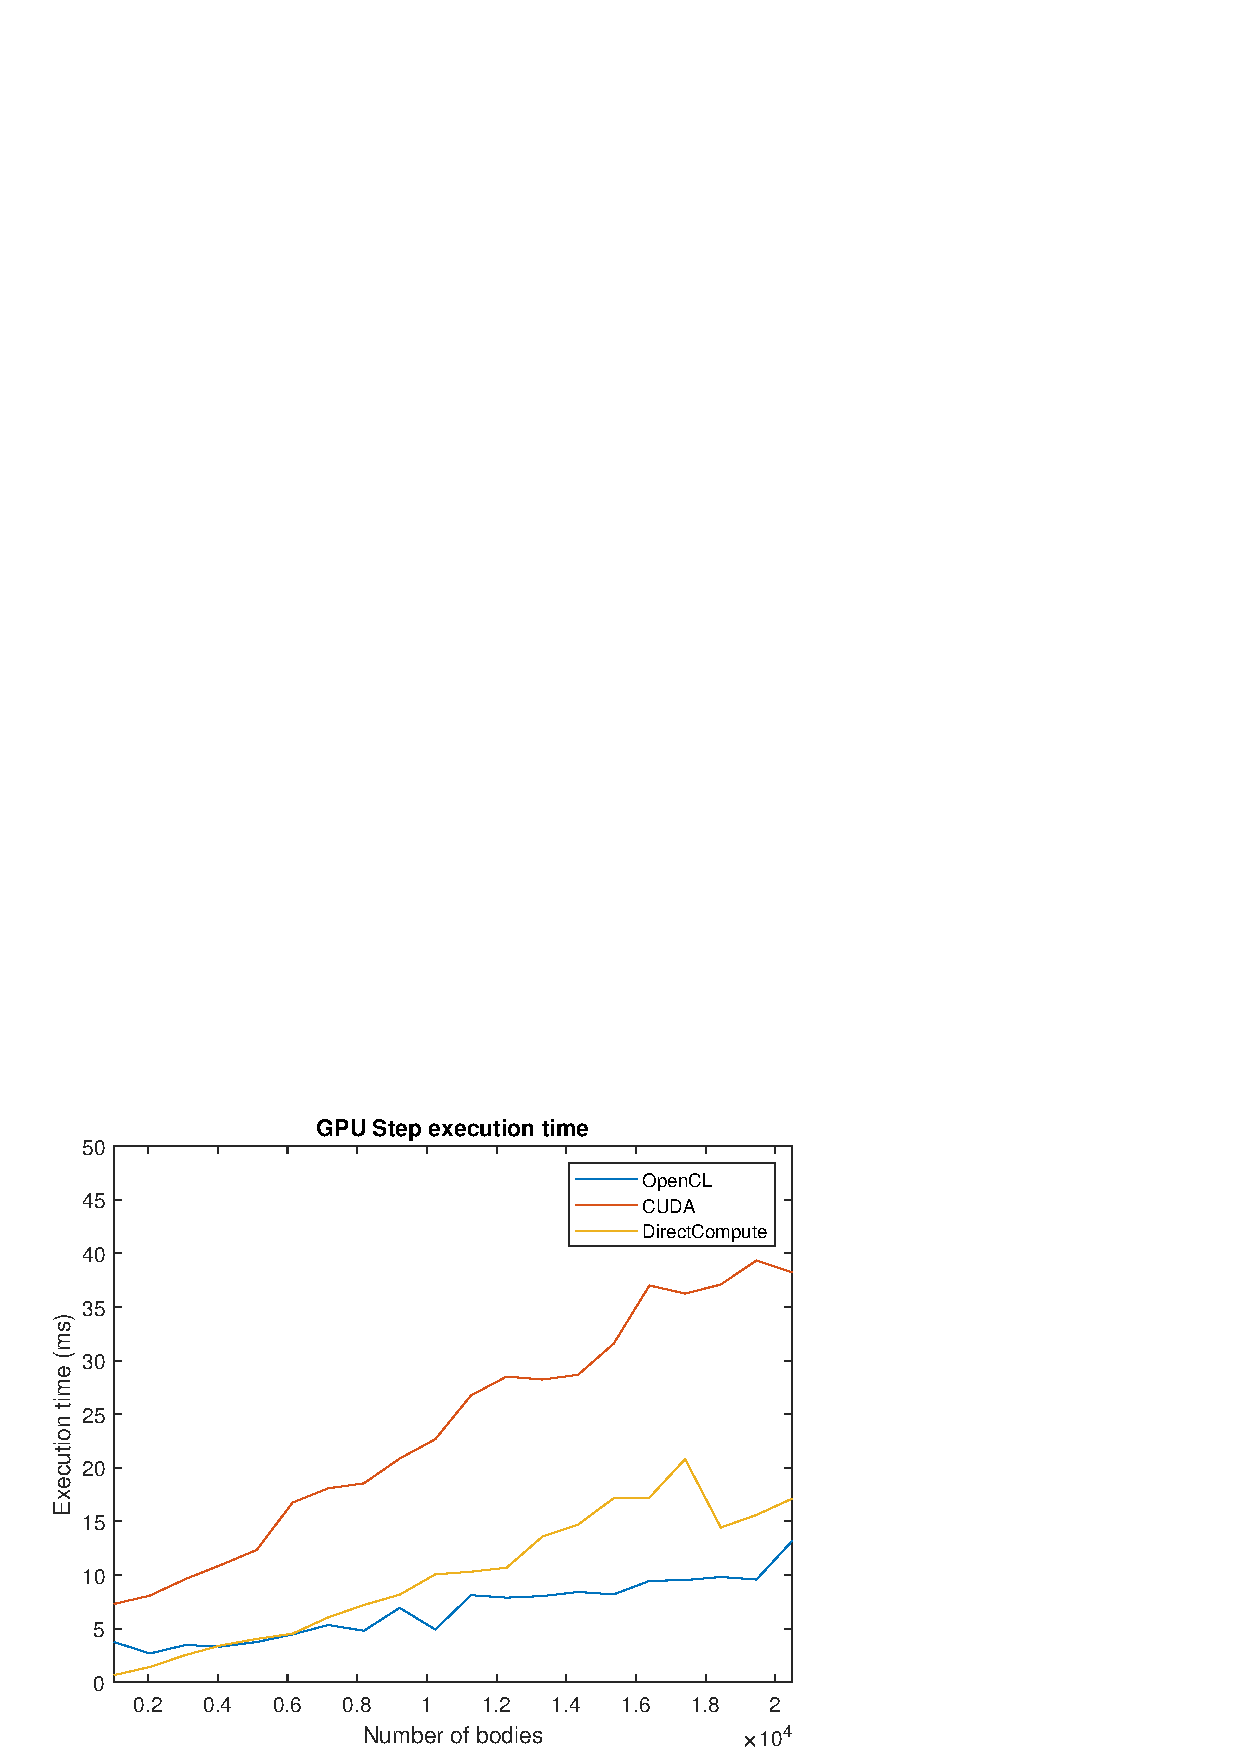
\includegraphics[width=0.8\textwidth]{Results/Figs/GPUStepExecutionTime.png}
    \caption{Execution time of the GPGPU step}
    \label{fig:GPUStepExecTime}
\end{figure}

To be able to compare what parts of the algorithm that was the most time consuming, the total execution time was broken apart and separated into 4 major parts:
\begin{itemize}
    \item \textbf{Build tree} - The time it takes for the CPU to for each timestep build the tree from the N-body system.
    \item \textbf{Calc. tree COM} - The time it takes for the CPU to traverse the tree and calculate each cells COM, total mass and the number of bodies in the subtree.
    \item \textbf{Flatten tree} - The time it takes for the CPU to flatten the pointer based tree into an container.
    \item \textbf{Step} - The time it takes to calculate the forces and update the positions. Executed on the GPU (apart from the sequential implementation).
\end{itemize}

The measured execution times for these parts are presented in figure \ref{fig:CUDAExecTime}, \ref{fig:OpenCLExecTime}, \ref{fig:DirectComputeExecTime} and \ref{fig:SeqExecTime}.

\begin{figure}[H]
    \centering
    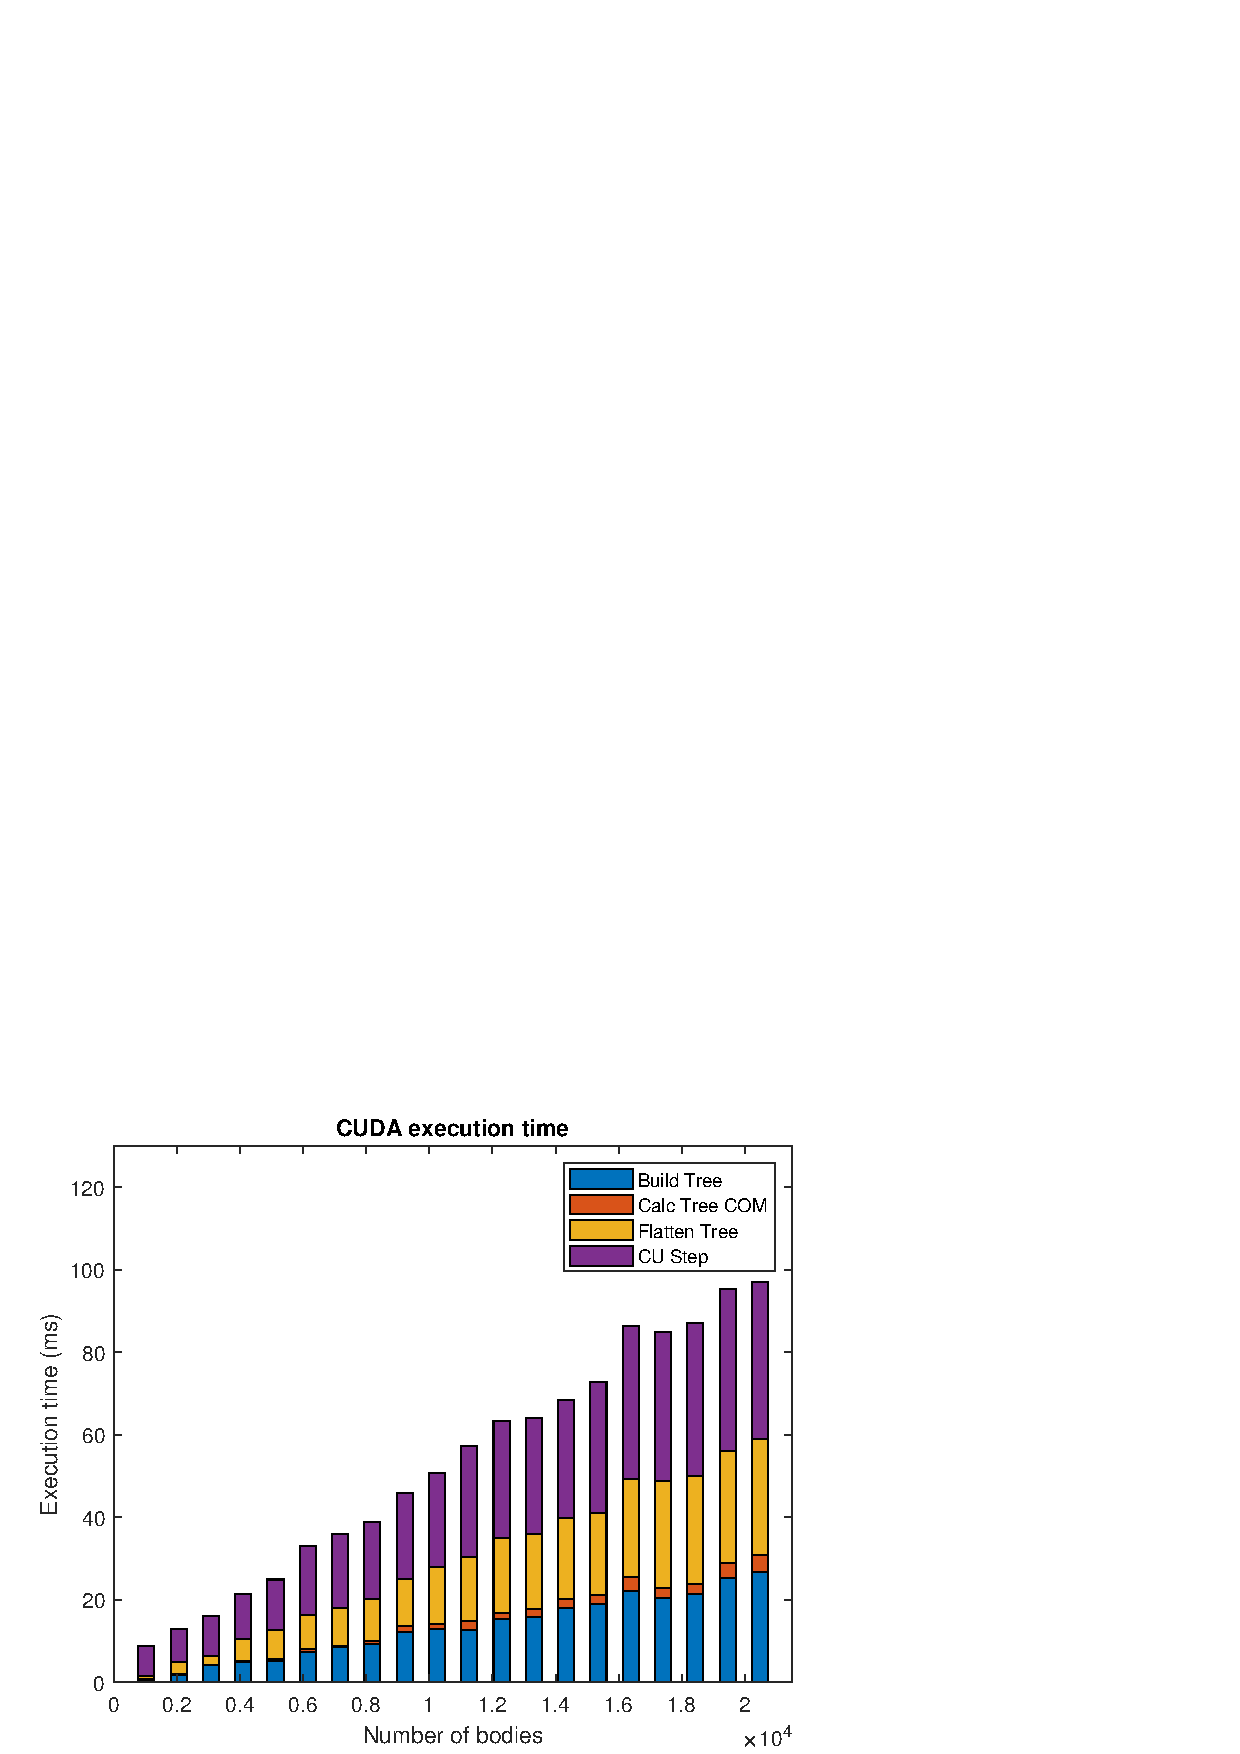
\includegraphics[width=.8\textwidth]{Results/Figs/CUDABarChart.png}
    \caption{CUDA execution time}
    \label{fig:CUDAExecTime}
\end{figure}

\begin{figure}[H]
    \centering
    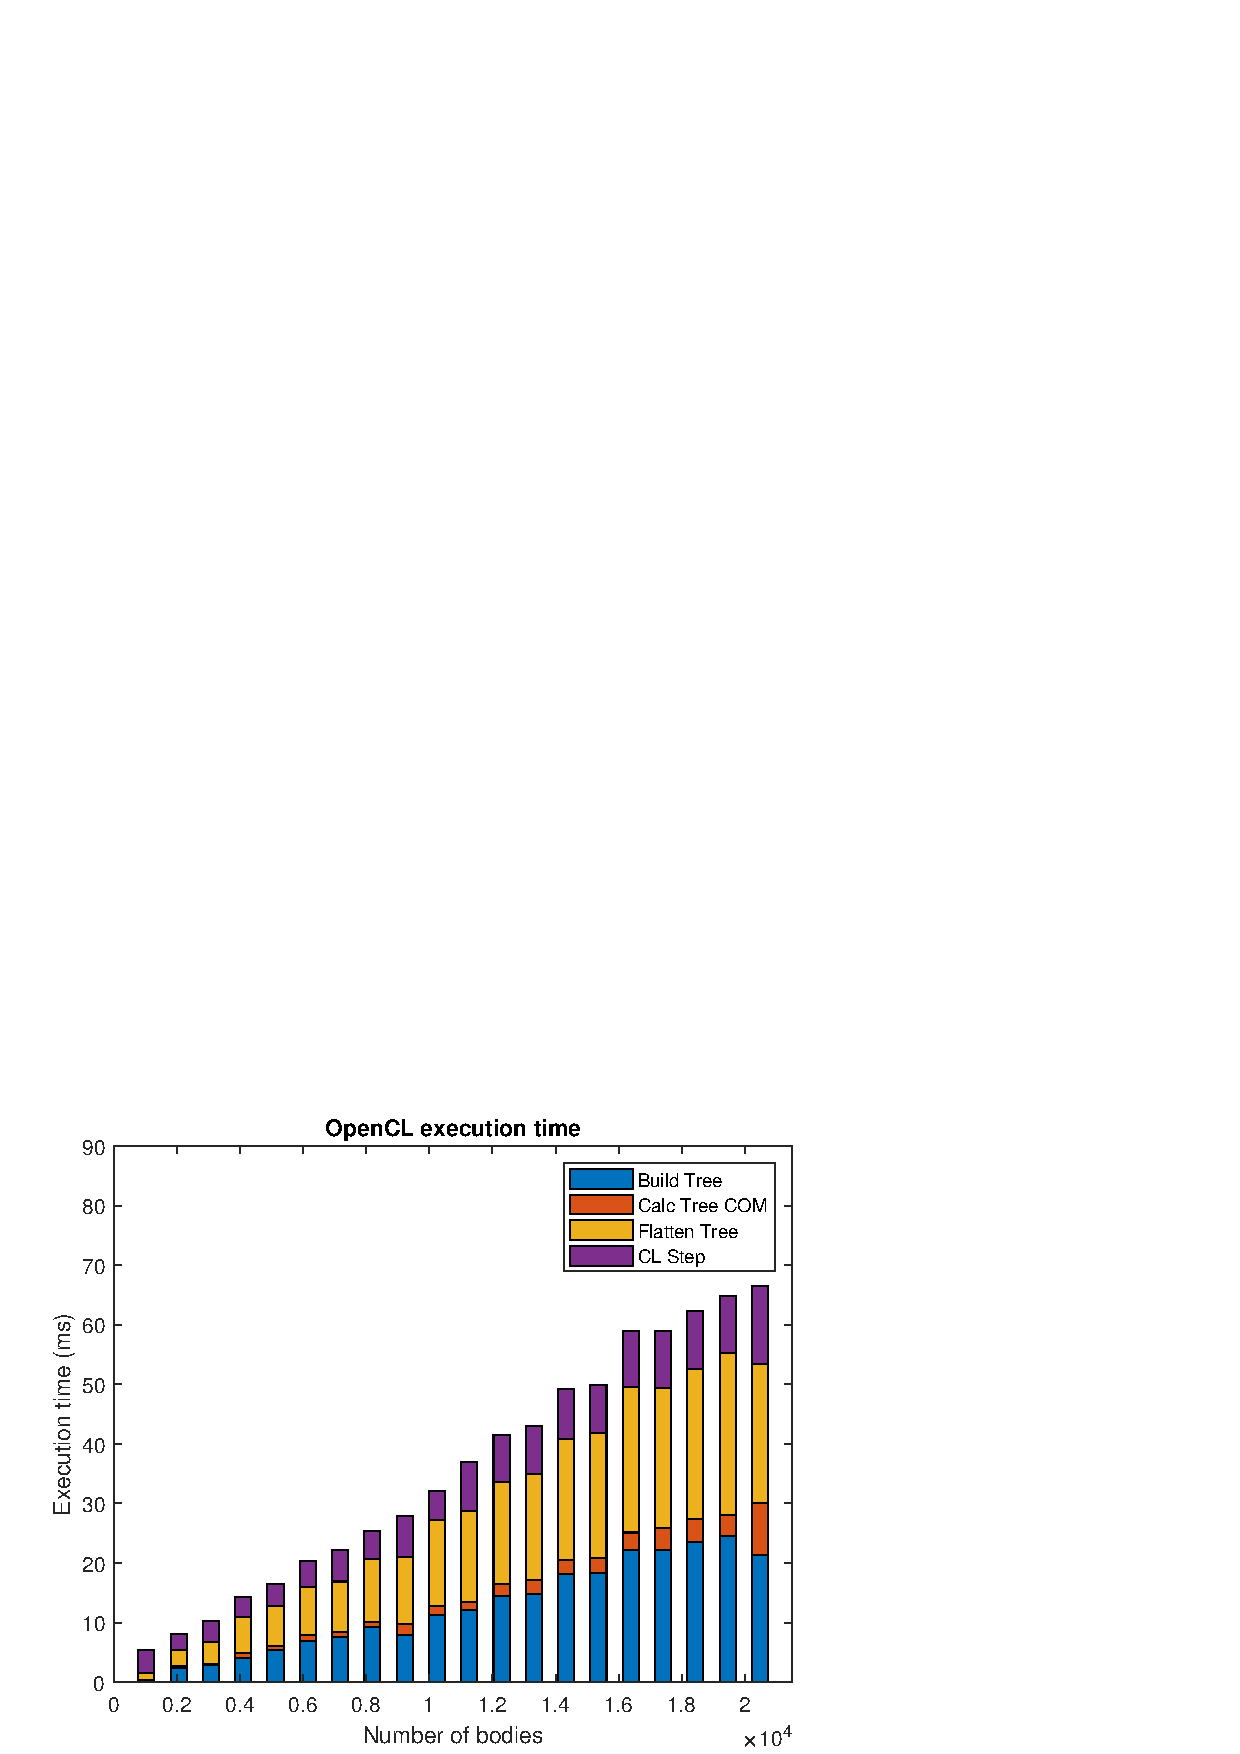
\includegraphics[width=.8\textwidth]{Results/Figs/OpenCLBarChart.png}
    \caption{OpenCL execution time}
    \label{fig:OpenCLExecTime}
\end{figure}

\begin{figure}[H]
    \centering  
    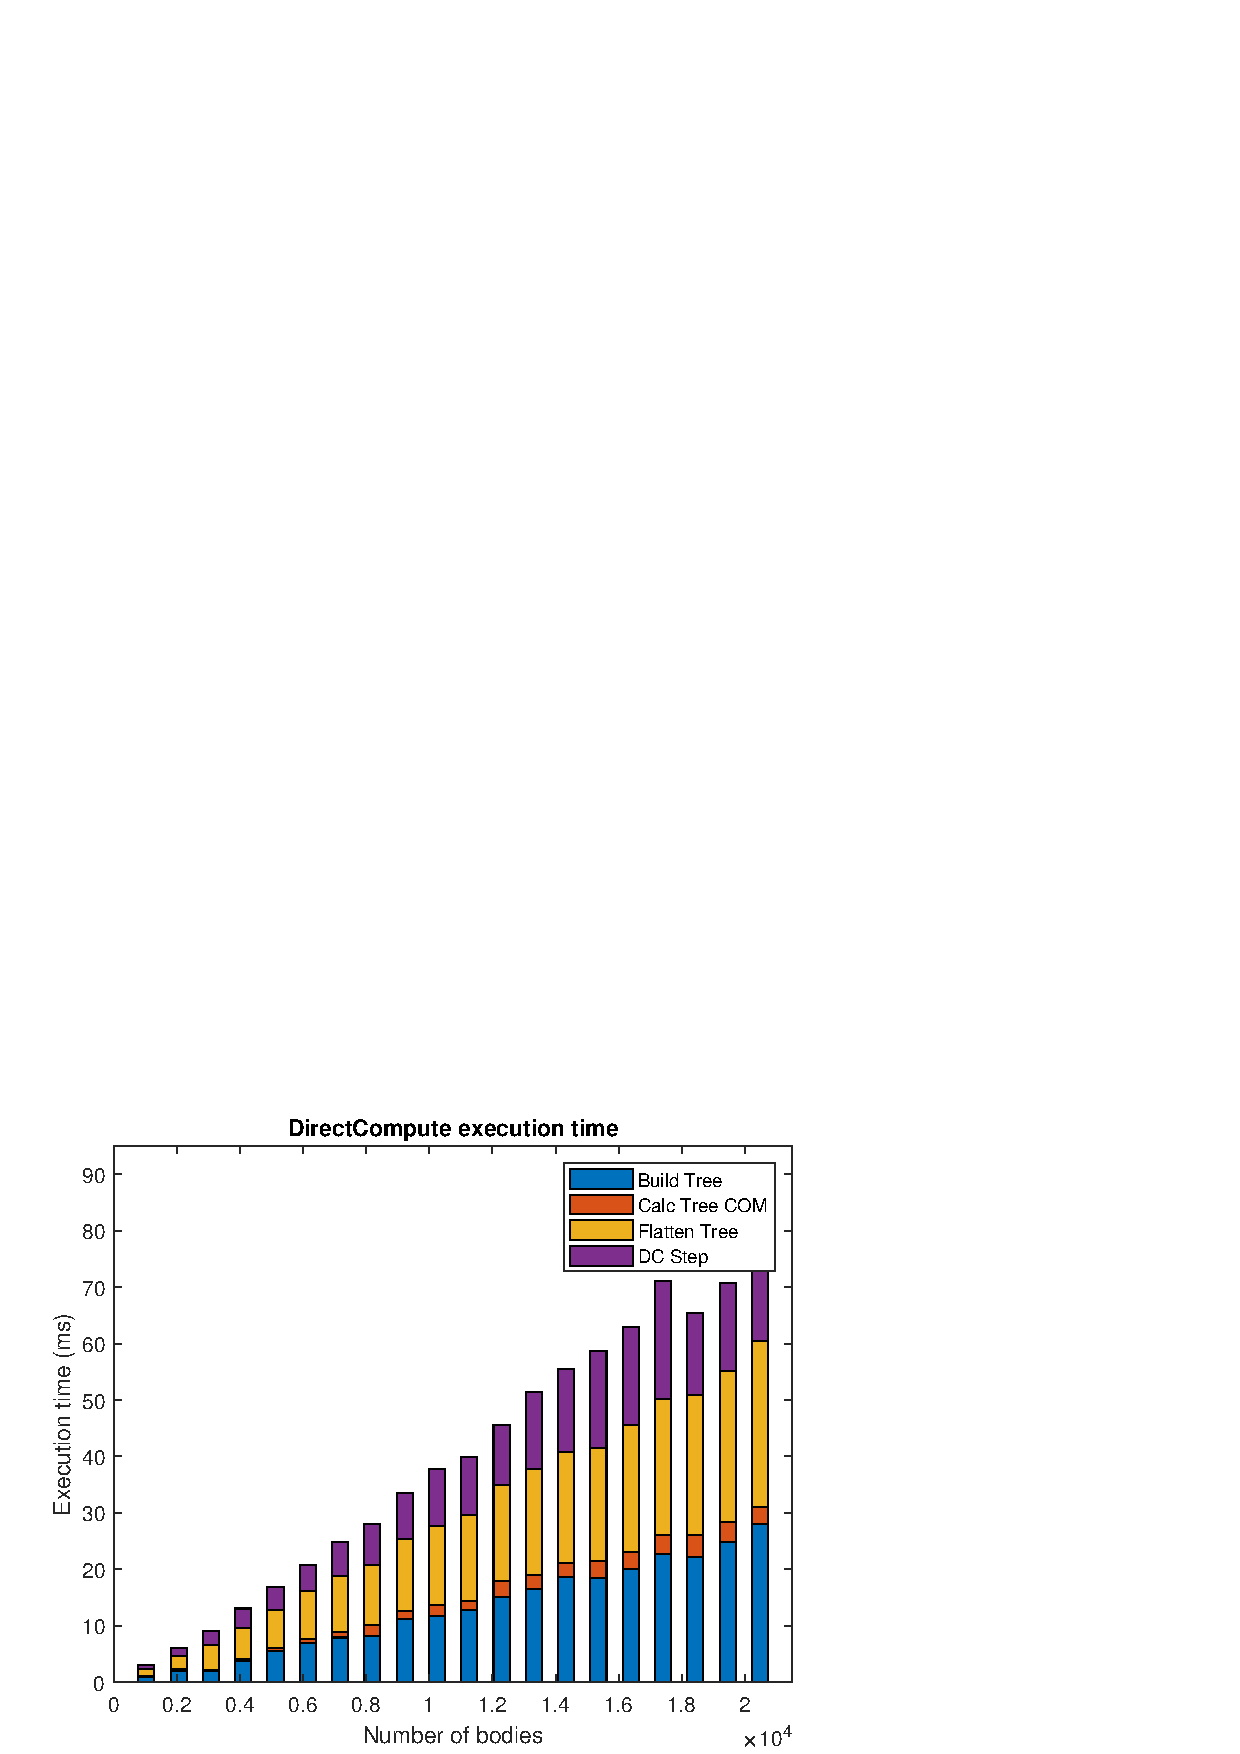
\includegraphics[width=.8\textwidth]{Results/Figs/DirectComputeBarChart.png}
    \caption{DirectCompute execution time}
    \label{fig:DirectComputeExecTime}
\end{figure}

\begin{figure}[H]
    \centering
    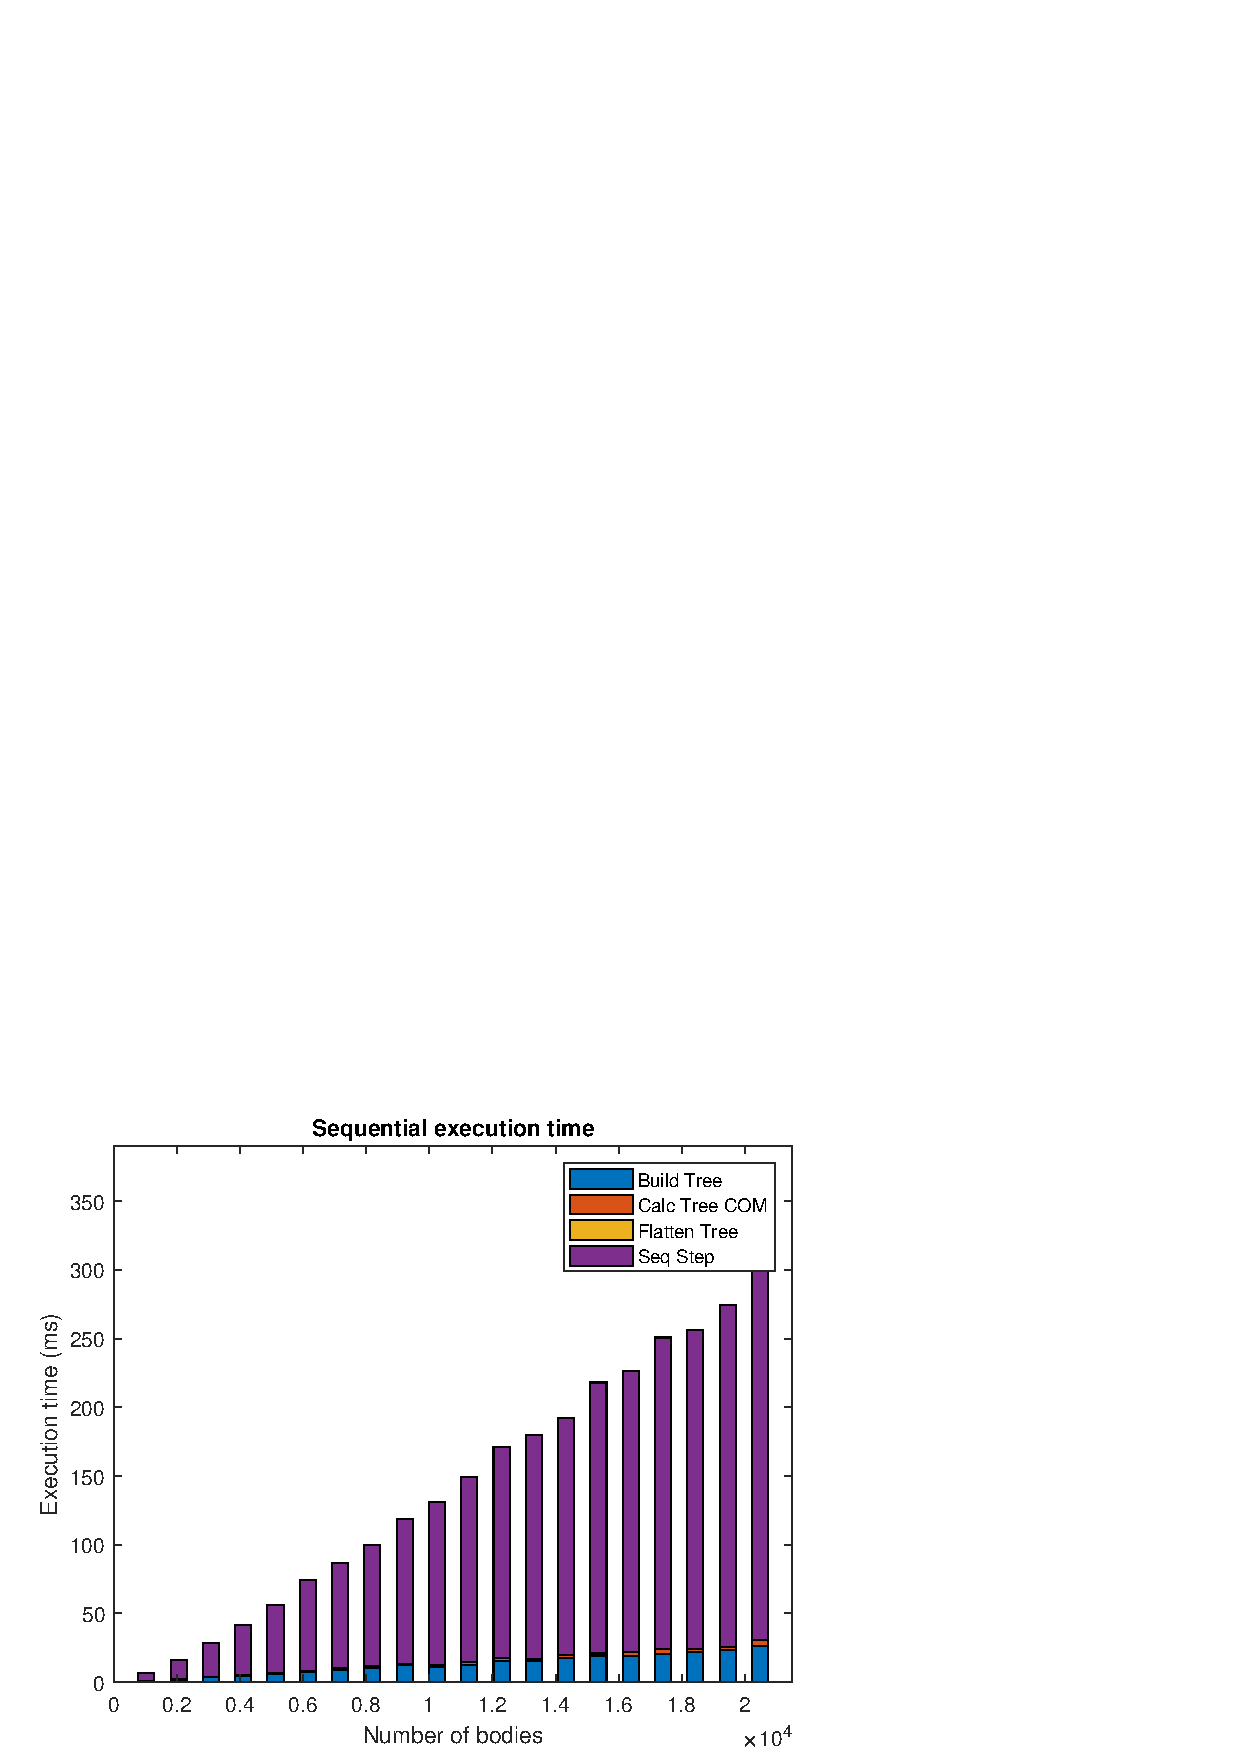
\includegraphics[width=.8\textwidth]{Results/Figs/SequentialBarChart.png}
    \caption{Sequential execution time}
    \label{fig:SeqExecTime}
\end{figure}


To be able to compare the performance difference when using buffers containing data structures and buffers containing class objects in CUDA, the execution time for both these cases was measured, the result is presented in figure \ref{fig:GraphCUDAStructVsClass}.

\begin{figure}[H]
    \centering
    \includegraphics[width=0.8\textwidth]{Results/Figs/CUDAStructVSClass.png}
    \caption{Execution time, CUDA Struct vs Class object buffers}
    \label{fig:GraphCUDAStructVsClass}
\end{figure}

\section{Features}

The features of the various frameworks given the specifications that are listed in table \ref{tab:SystemSpecs} are listed in table \ref{tab:FrameworkFeatures} \cite{CudaDOCS}\cite{DCGuide}\cite{DCGuideNvidia}. SkePU is unlisted since the features depends on the choice of backend. 

The table lists the feature specifications for OpenCL 1.2, which is the newest Nvidia version and was used in this implementation.
OpenCL 2.0 brought major differences which makes it a strong candidate feature-wise compared to CUDA, and OpenCL 2.0 supports the OpenCL C++ kernel language, which thus makes it possible to create and utilize classes in the kernel. OpenCL 2.0 also adds the ability to launch kernels from within kernels, i.e Dynamic parallelism.

Furthermore, the table lists specifications for DirectCompute when run on Direct3D 11.x hardware and thus using the CS 5.0 model. Older hardware (Direct3D 10.x) only supports the CS 4.0 model which adds some further restrictions. 
The main differences is that while CS 5.0 supports a max number of 1024 threads per group, CS 4.0 only supports 768. CS 4.0 does not support 3D grid dimensions, and have no atomic operations, scatter operations and does not support double precision. Finally, while CS 5.0 supports eight UAVs which can be bound to a shader, CS 4.0 only allows for one UAV.

\begin{table}[H]

    % Features
    \begin{tabularx}{\textwidth}{ |c|c|c|X| }
        \hline
        \rowcolor{gray}
        \multicolumn{4}{|c|}{\textbf{Features}}\\ \hline
      
                                            & \textbf{CUDA}                      & \textbf{OpenCL (1.2)}        & \textbf{DirectCompute (D3D11)}    \\ \hline
        \textbf{Kernel Language}            & \cellcolor{green}Cuda C/C++        & \cellcolor{green}OpenCL C    & \cellcolor{green}HLSL             \\ \hline
        \textbf{Kernel classes}             & \cellcolor{green}Yes               & \cellcolor{red}No            & \cellcolor{red}No                 \\ \hline
        \textbf{Kernel recursion}           & \cellcolor{green}Yes               & \cellcolor{red}No            & \cellcolor{red}No                 \\ \hline
        \textbf{Dynamic parallelism}        & \cellcolor{green}Yes               & \cellcolor{red}No            & \cellcolor{red}No                 \\ \hline
        \hline
        \textbf{Class object buffers}       & \cellcolor{green}Yes               & \cellcolor{red}No            & \cellcolor{red}No                 \\ \hline
        \textbf{Structured buffers}         & \cellcolor{green}Yes               & \cellcolor{green}Yes         & \cellcolor{green}Yes              \\ \hline
        \hline
        \textbf{Warp size}                  & \cellcolor{green}32                & \cellcolor{green}32          & \cellcolor{green}32               \\ \hline
        \textbf{Atomic Operations}          & \cellcolor{green}Yes               & \cellcolor{green}Yes         & \cellcolor{green}Yes              \\ \hline
        \textbf{64 bit precision}           & \cellcolor{green}Yes               & \cellcolor{green}Yes         & \cellcolor{green}Yes              \\ \hline
        \textbf{3D Grid Dimensions}         & \cellcolor{green}Yes               & \cellcolor{green}Yes         & \cellcolor{green}Yes              \\ \hline
        \textbf{No. Threads/group}          & \cellcolor{green}1024              & \cellcolor{green}1024        & \cellcolor{green}1024             \\ \hline 
        \hline
        \textbf{Thread local mem.}          & \cellcolor{green}512 KB            & \cellcolor{gray}-            & \cellcolor{gray}-                 \\ \hline
        \textbf{Shared mem./group}          & \cellcolor{green}48 KB             & \cellcolor{green}42 KB       & \cellcolor{green}16 KB            \\ \hline
        \textbf{Constant mem. size}         & \cellcolor{green}64 KB             & \cellcolor{green}64 KB       & \cellcolor{green}64 KB            \\ \hline
        \textbf{Group synchronization}      & \cellcolor{green}Yes               & \cellcolor{green}Yes         & \cellcolor{green}Yes              \\ \hline
        \textbf{Gather operations}          & \cellcolor{green}Yes               & \cellcolor{green}Yes         & \cellcolor{green}Yes              \\ \hline
        \textbf{Scatter operations}         & \cellcolor{green}Yes               & \cellcolor{green}Yes         & \cellcolor{green}Yes              \\ \hline
        
    \end{tabularx}

\caption{\label{tab:FrameworkFeatures} Framework features given the specifications listed in table \ref{tab:SystemSpecs}.}
\end{table}


\section{Portability}

This section will describe the portability of the various frameworks. Portability limitations for each of the evaluated frameworks and the percentage of devices that are able to utilize the frameworks are presented, summarized from market share statistics for operating systems and GPU vendors. 

\vskip .5em
\noindent \textbf{OpenCL} was developed with portability in mind, OpenCL is able to be utilized on systems with compatible hardware. Since OpenCL is able to perform parallel computations on a wide variety of devices, the portability of the framework is high and works on most systems.

\vskip .5em
\noindent \textbf{CUDA} only available on Nvidia GPUs, newer than the 8800 series, codenamed G80 (2006). Cuda is obtained by downloading and installing the Nvidia CUDA Toolkit and is available on all major operating systems.

\vskip .5em
\noindent \textbf{DirectCompute} which is a part of the DirectX suite, only works on Microsoft Windows systems with Direct3D 10.0 and up. 

\vskip 1em
The market share of the most popular desktop and laptop system operating systems Windows, OSX and Linux, are presented in figure \ref{fig:OSMarketShare} (Q1 2018) \cite{Marketshare}. The market share of the GPU vendors AMD and Nvidia are listed in figure \ref{fig:GPUMarketShare} (Q4 2017) \cite{GPUMarketshare}.
% ===================================== % 
% ====== OPERATING SYSTEM STATS ====== %
% https://netmarketshare.com/operating-system-market-share.aspx?options=%7B%22filter%22%3A%7B%22%24and%22%3A%5B%7B%22deviceType%22%3A%7B%22%24in%22%3A%5B%22Desktop%2Flaptop%22%5D%7D%7D%5D%7D%2C%22dateLabe%l%22%3A%22Trend%22%2C%22attributes%22%3A%22share%22%2C%22group%22%3A%22platform%22%2C%22sort%22%3A%7B%22share%22%3A-1%7D%2C%22id%22%3A%22platformsDesktop%22%2C%22dateInterval%22%3A%22Monthly%22%2C%22dateStart%22%3A%222017-03%22%2C%22dateEnd%22%3A%222018-02%22%2C%22segments%22%3A%22-1000%22%7D


% GPU Market share stats
% https://wccftech.com/nvidia-amd-discrete-gpu-market-share-report-q3-2017/

% ===================================== % 

\begin{figure}[H]
    \centering
    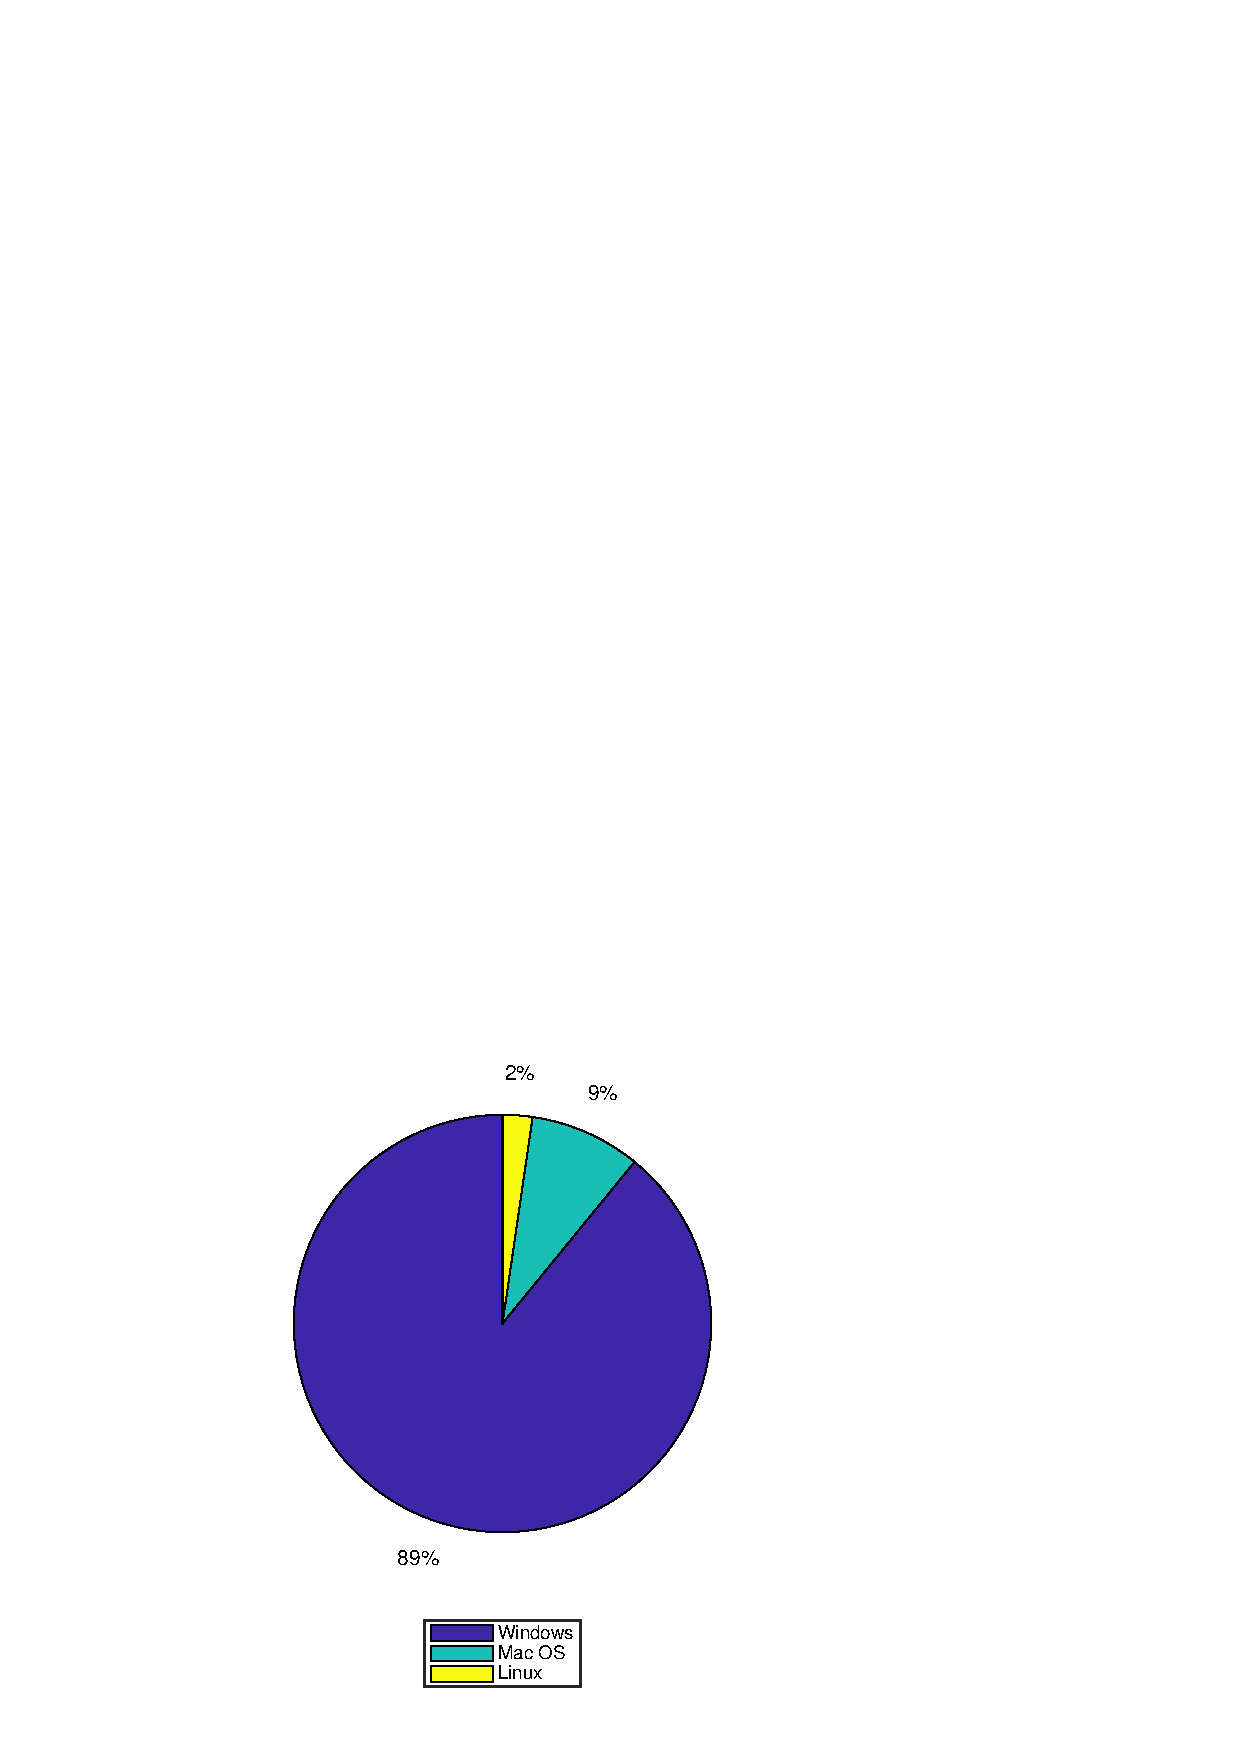
\includegraphics[width=.8\textwidth]{Results/Figs/OSMarketShare.png}
    \caption{Operating system market share (Q1 2018)}
    \label{fig:OSMarketShare}
\end{figure}

\begin{figure}[H]
    \centering
    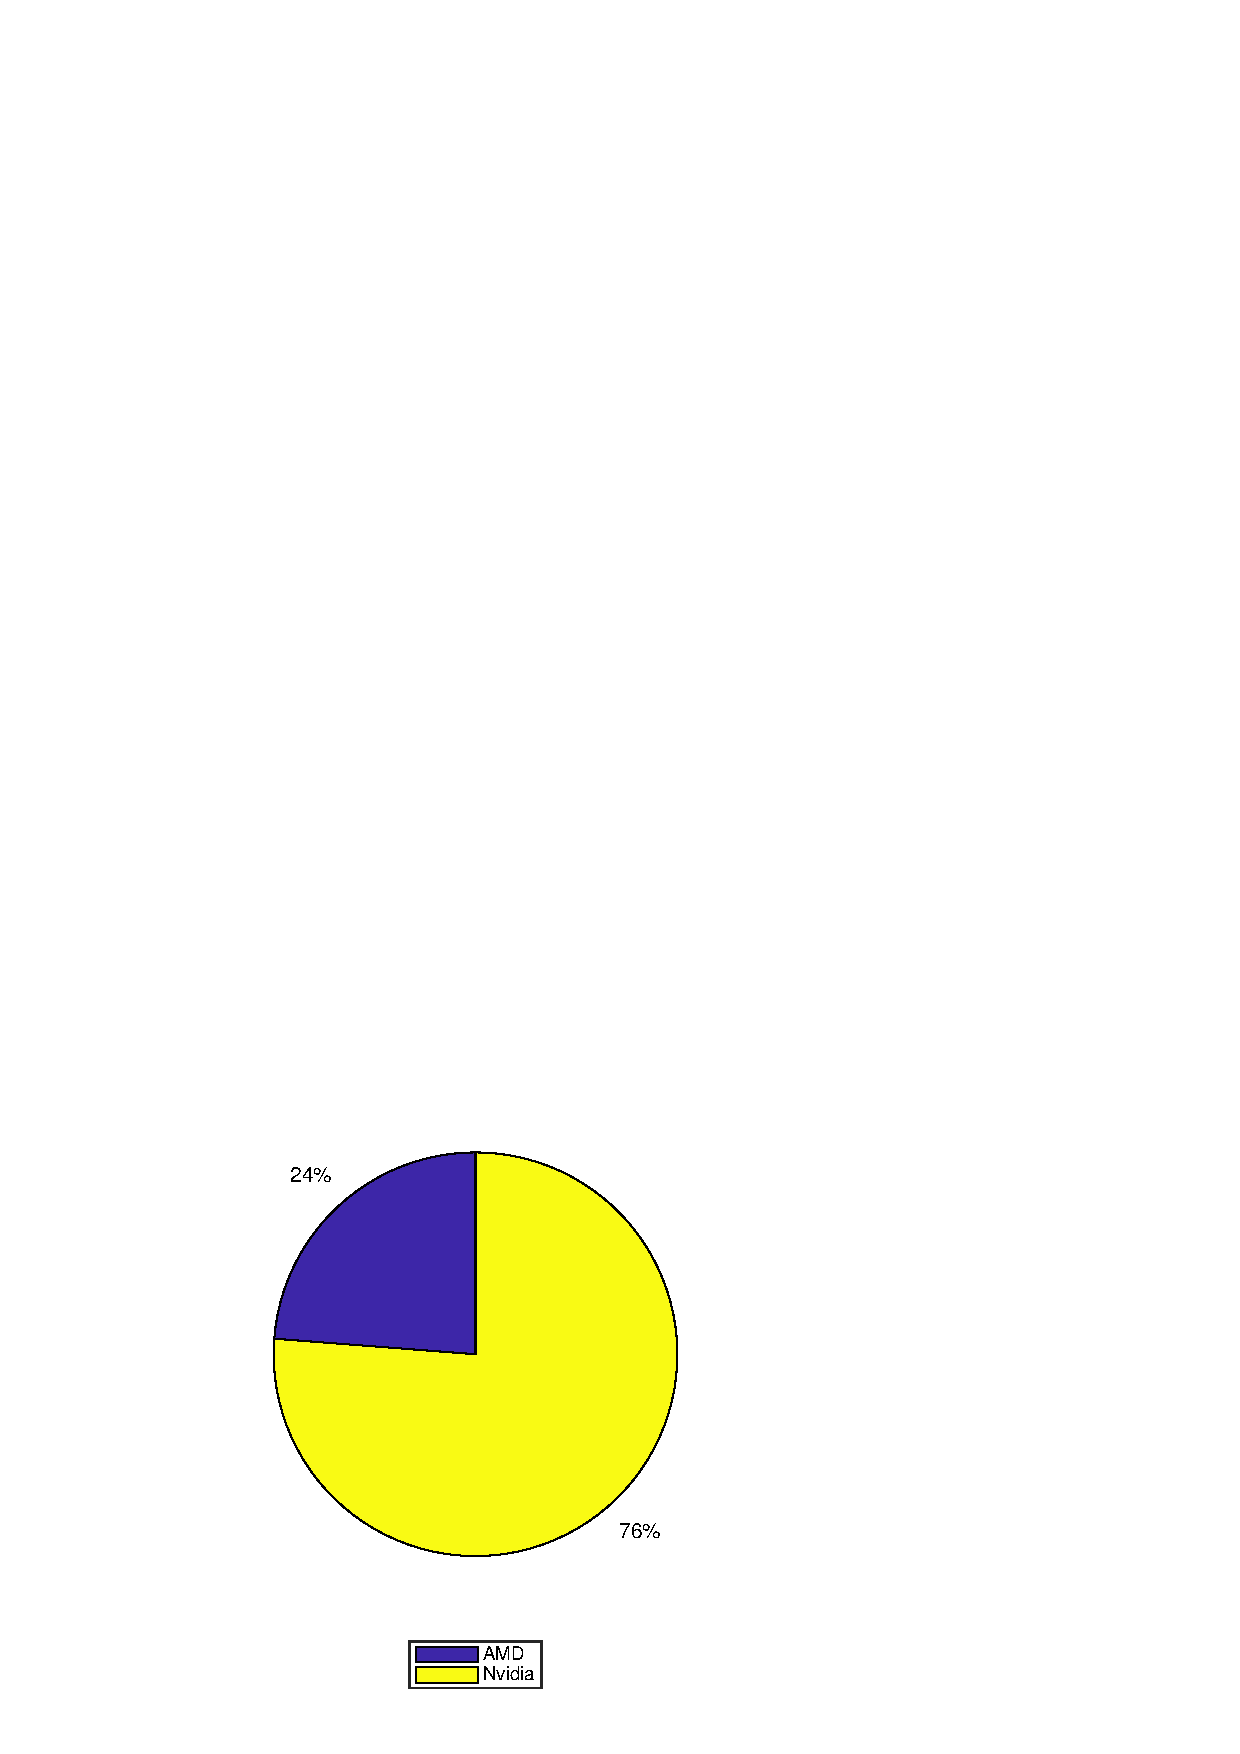
\includegraphics[width=.8\textwidth]{Results/Figs/GPUMarketShare.png}
    \caption{AMD and Nvidia market share (Q4 2017)}
    \label{fig:GPUMarketShare}
\end{figure}

\section{Code complexity}

Appendix \ref{appendix:CUDAVecAdd}, \ref{appendix:OpenCLVecAdd}, \ref{appendix:DirectComputeVecAdd} and \ref{appendix:SkepuVecAdd} lists full working code examples which performs a simple vector addition according to 
$\boldsymbol A + \boldsymbol B = \boldsymbol C = (a_1 + b_1, a_2 + b_2, ... , a_n +b_n)$ in CUDA, OpenCL, DirectCompute and SkePU accordingly. To measure the code complexity, these implementations was tested using the freeware software SourceMonitor \cite{SourceMonitor}. The results of these measurements are presented in table \ref{tab:VecAddMetrics}.


\begin{table}[H] 
    % General
    \begin{tabularx}{\textwidth}{ |X|X| }
      \hline
      \rowcolor{gray}
      \multicolumn{2}{|c|}{\textbf{CUDA Vector Addition}}\\ \hline
      \textbf{Lines}            & 45 \\ \hline
      \textbf{Statements}               & 38 \\ \hline
      \textbf{Max Complexity}           & 4 \\ \hline
      \textbf{Avg. Complexity}          & 0.97 \\ \hline
      \textbf{Max Depth}                & 3 \\ \hline
      \textbf{Avg. Depth}               & 0.97 \\ \hline
    \end{tabularx}
    \begin{tabularx}{\textwidth}{ |X|X| }
      \hline
      \rowcolor{gray}
      \multicolumn{2}{|c|}{\textbf{OpenCL Vector Addition}}\\ \hline
      \textbf{Lines}                    & 68 \\ \hline
      \textbf{Statements}               & 42 \\ \hline
      \textbf{Max Complexity}           & 4 \\ \hline
      \textbf{Avg. Complexity}          & 2.5 \\ \hline
      \textbf{Max Depth}                & 3 \\ \hline
      \textbf{Avg. Depth}               & 0.95 \\ \hline
    \end{tabularx}
    \begin{tabularx}{\textwidth}{ |X|X| }
      \hline
      \rowcolor{gray}
      \multicolumn{2}{|c|}{\textbf{DirectCompute Vector Addition}}\\ \hline
      \textbf{Lines}                    & 241 \\ \hline
      \textbf{Statements}               & 144 \\ \hline
      \textbf{Max Complexity}           & 9 \\ \hline
      \textbf{Avg. Complexity}          & 4.14 \\ \hline
      \textbf{Max Depth}                & 5 \\ \hline
      \textbf{Avg. Depth}               & 1.31 \\ \hline
    \end{tabularx}
    \begin{tabularx}{\textwidth}{ |X|X| }
      \hline
      \rowcolor{gray}
      \multicolumn{2}{|c|}{\textbf{SkePU Vector Addition}}\\ \hline
      \textbf{Lines}                    & - \\ \hline
      \textbf{Statements}               & - \\ \hline
      \textbf{Max Complexity}           & - \\ \hline
      \textbf{Avg. Complexity}          & - \\ \hline
      \textbf{Max Depth}                & - \\ \hline
      \textbf{Avg. Depth}               & - \\ \hline
    \end{tabularx}
    \caption{\label{tab:VecAddMetrics} Metrics for the vector addition examples listed in Appendix \ref{appendix:CUDAVecAdd}, \ref{appendix:OpenCLVecAdd}, \ref{appendix:DirectComputeVecAdd} and \ref{appendix:SkepuVecAdd}.}
\end{table}








